%%%%%%%% ICML 2024 EXAMPLE LATEX SUBMISSION FILE %%%%%%%%%%%%%%%%%

\documentclass{article}

% Recommended, but optional, packages for figures and better typesetting:
\usepackage{xurl}
\usepackage{hyperref}
\usepackage{microtype}
\usepackage{graphicx}
\usepackage{subfigure}
\usepackage{booktabs} % for professional tables
\usepackage{placeins}

% hyperref makes hyperlinks in the resulting PDF.
% If your build breaks (sometimes temporarily if a hyperlink spans a page)
% please comment out the following usepackage line and replace
% \usepackage{icml2024} with \usepackage[nohyperref]{icml2024} above.
\usepackage{hyperref}


% Attempt to make hyperref and algorithmic work together better:
\newcommand{\theHalgorithm}{\arabic{algorithm}}

% Use the following line for the initial blind version submitted for review:
\usepackage[accepted]{icml2024}

% If accepted, instead use the following line for the camera-ready submission:
% \usepackage[accepted]{icml2024}

% For theorems and such
\usepackage{amsmath}
\usepackage{amssymb}
\usepackage{mathtools}
\usepackage{amsthm}
\usepackage{subcaption}

% if you use cleveref..
\usepackage[capitalize,noabbrev]{cleveref}

%%%%%%%%%%%%%%%%%%%%%%%%%%%%%%%%
% THEOREMS
%%%%%%%%%%%%%%%%%%%%%%%%%%%%%%%%
\theoremstyle{plain}
\newtheorem{theorem}{Theorem}[section]
\newtheorem{proposition}[theorem]{Proposition}
\newtheorem{lemma}[theorem]{Lemma}
\newtheorem{corollary}[theorem]{Corollary}
\theoremstyle{definition}
\newtheorem{definition}[theorem]{Definition}
\newtheorem{assumption}[theorem]{Assumption}
\theoremstyle{remark}
\newtheorem{remark}[theorem]{Remark}

% Todonotes is useful during development; simply uncomment the next line
%    and comment out the line below the next line to turn off comments
%\usepackage[disable,textsize=tiny]{todonotes}
\usepackage[textsize=tiny]{todonotes}


% The \icmltitle you define below is probably too long as a header.
% Therefore, a short form for the running title is supplied here:
\icmltitlerunning{AI and Decision Making for Medicine and Therapy: Final Project}

\begin{document}

\twocolumn[
\icmltitle{AI-based Early Prediction of Sepsis from Time-Labeled Clinical Data}

% It is OKAY to include author information, even for blind
% submissions: the style file will automatically remove it for you
% unless you've provided the [accepted] option to the icml2024
% package.

% List of affiliations: The first argument should be a (short)
% identifier you will use later to specify author affiliations
% Academic affiliations should list Department, University, City, Region, Country
% Industry affiliations should list Company, City, Region, Country

% You can specify symbols, otherwise they are numbered in order.
% Ideally, you should not use this facility. Affiliations will be numbered
% in order of appearance and this is the preferred way.
\icmlsetsymbol{equal}{*}

\begin{icmlauthorlist}
\icmlauthor{Lee Chen}{equal,yyy}
\icmlauthor{Samir Kadariya}{equal,yyy}
\icmlauthor{Shauna Kwag}{equal,yyy}
\icmlauthor{Pari Latawa}{equal,yyy}
\icmlauthor{Phoenix Wu}{equal,yyy}
\icmlauthor{Richard Zhu}{equal,yyy}

%\icmlauthor{}{sch}
%\icmlauthor{}{sch}
\end{icmlauthorlist}

\icmlaffiliation{yyy}{Department of EECS, MIT, Cambridge, MA, USA}

\icmlcorrespondingauthor{Firstname1 Lastname1}{first1.last1@xxx.edu}
\icmlcorrespondingauthor{Firstname2 Lastname2}{first2.last2@www.uk}
\icmlcorrespondingauthor{Firstname2 Lastname2}{first2.last2@www.uk}


% You may provide any keywords that you
% find helpful for describing your paper; these are used to populate
% the "keywords" metadata in the PDF but will not be shown in the document
\icmlkeywords{Machine Learning, ICML}

\vskip 0.3in
]

% this must go after the closing bracket ] following \twocolumn[ ...

% This command actually creates the footnote in the first column
% listing the affiliations and the copyright notice.
% The command takes one argument, which is text to display at the start of the footnote.
% The \icmlEqualContribution command is standard text for equal contribution.
% Remove it (just {}) if you do not need this facility.

%\printAffiliationsAndNotice{}  % leave blank if no need to mention equal contribution
%\printAffiliationsAndNotice{\icmlEqualContribution} % otherwise use the standard text.

\begin{abstract}

Early prediction of sepsis is critical for reducing mortality but remains difficult due to the heterogeneous and sparse nature of clinical time-series data. Using the 2019 PhysioNet Challenge framework—which evaluates models using a utility function emphasizing timely alerts—we compare three approaches for early sepsis detection against a logistic regression baseline: an autoencoder with k-nearest neighbors, an LSTM, and a Transformer. The challenge’s preprocessing pipeline includes forward-fill and population-mean imputation, missingness indicators, and optional temporal feature augmentations. Using a dataset of 11,000 patients, models with strong temporal inductive biases substantially outperform static or representation-learning methods. The Transformer achieved the highest normalized utility (0.578) with strong early-warning capability but a high false-positive rate, followed by the LSTM (0.261), while the autoencoder + k-NN model performed poorly (0.04). These results underscore the importance of modeling long-range physiological trajectories and highlight attention-based architectures as particularly effective for clinically meaningful early sepsis prediction.

\end{abstract}

\section{Introduction}
\label{submission}

Sepsis is a life-threatening immune response to infection. It occurs when the immune system causes an extreme, systemic full-body response with widespread inflammation and vascular permeability leading to tissue damage, organ failure, and even death.

Many sources of infection can lead to sepsis. Among them are pneumonia in infectious lung disease, catheter-related infections, and abdominal infections like appendicitis. These diseases can be nosocomial, meaning acquired in-hospital. Moreover, in-hospital patients often have comorbidities that can increase susceptibility to infection and resulting sepsis. Treatments as well can increase infection risk, with catheterization and the difficulty of maintaining a sterile environment being some factors. As a result, it would be reasonable to focus on predicting which patients could develop sepsis and when based on vital signs recorded periodically during a hospital stay.

Indeed, in the United States, 1.7 million people develop sepsis each year with 270 thousand of those cases being fatal \cite{hurst2020cost}. Further, sepsis contributes to over one-third of all patient deaths in United States hospitals \cite{hurst2020cost}. These statistics highlight sepsis as a key obstacle to improving patient outcomes during in-hospital stays and suggest that addressing sepsis as a medical issue is both warranted and upfront.

Sepsis also poses a financial burden. It is the number one inpatient hospital expense in the United States, costing 23.7 billion dollars annually \cite{hurst2020cost}. And given the medical and financial imperatives it becomes important to understand why sepsis outcomes depend on time.

During early stages of sepsis, prompt treatment with antibiotics and IV fluids often leads to full recovery. While inflammation may manifest some symptoms, including fever and/or discomfort, the more serious symptoms like organ dysfunction and blood pressure drop have not yet occurred and led to more lasting effects. In studies where mortality was plotted against antibiotic administration time, this phenomenon can be observed \cite{im2022timetoantibiotics}. The longer the time to antibiotic administration, the greater the mortality rate. However, mortality increases gradually over time and reaches a very high rate only in sepsis patients but not the control and only at later times of antibiotic administration. That would suggest it is indeed possible to address the challenge of sepsis with early detection and prophylactic treatment and/or surveillance.

Unfortunately, current clinical approaches to sepsis often are ineffective. Diagnosis of the systemic inflammatory response syndrome (SIRS) is done based on heart rate, respiratory rate, temperature, and WBC abnormalities, but is often not specific enough \cite{kaukonen2015sirs, singer2016sepsis3, beesley2015neednewdef}. General inflammation from any cause can lead to over-diagnosis, while some true sepsis cases are missed as well. Another clinical assessment is the sequential organ failure assessment (SOFA) which determines the health of six organ systems. By the time a decline in organ function is observed, however, sepsis has already caused damage to the patient’s body. Thus, treatment would shift to damage control.

Early detection with machine learning models instead provides a promising avenue for prophylactic treatment and/or surveillance. It does not depend on heuristics about biomarkers with arbitrary cutoffs that are ineffective at improving patient outcomes to the extent that they are warranted. The caveat is that machine learning work often focuses on statistics that do not necessarily represent clinical outcomes. So, it followed that a project to predict early sepsis would best use a utility metric rewarding early detection and avoiding false alarms.

These challenges and the idea for machine learning based approaches led to the 2019 PhysioNet Challenge \cite{singer2016sepsis3, reyna2019early, goldberger2000physionet}. More accurate, early, and actionable sepsis prediction models would benefit the medical community and dramatically improve patient survival.

Since physiological changes over time are heterogeneous, irregular, noisy, sparse, gradual, nonlinear, and confounding to heuristics and clinicians alike at the moment, a project determining the utility of various models was conducted on sepsis time-series data.

\section{Methods}

\subsection{Baseline: Logistic Regression}
As a simple and interpretable baseline, we trained a logistic regression model using only missingness patterns in the data. This approach ignores all physiological values and looks solely at whether each feature is recorded at a given hour. This approach reflects the intuition that the recorded data can carry information about patient deterioration. A logistic regression approach allows linear coefficients to directly indicate how the absence or presence of specific measurements shifts the estimated sepsis risk. The output can be interpreted as a “probability” score. An AUROC of 0.5996 and an AUPRC of 0.0298 were achieved. The logistic model did not do very well with a utility of about 0.10, likely because it was unable to capture complex physiological or evolving patterns.

\subsection{Datasets}

\subsubsection{Dataset Pre-Processing}

The PhysioNet Challenge 2019 dataset requires extensive preprocessing to handle missing data and prepare temporal features for model training. The dataset comprises 11,000 patients split into training (5,000 patients), validation (1,000 patients), and test (5,000 patients) sets as shown in Figure~\ref{fig:dataset_splits}. Each patient record consists of hourly measurements across 40 clinical features including vital signs (heart rate, temperature, respiratory rate), blood pressure metrics (systolic, diastolic, mean arterial pressure), oxygenation parameters (SpO$_2$, EtCO$_2$), and various laboratory values. The temporal sequences vary in length across patients, reflecting different lengths of ICU stays ranging from several hours to multiple days. The dataset exhibits severe class imbalance, with only 8.28\% of training patients developing sepsis (414 of 5,000 patients). This imbalance is even more pronounced at the timestep level, as the majority of hourly measurements occur before sepsis onset. The validation and test sets exhibit similar imbalance ratios (approximately 6--8\% sepsis prevalence), reflecting the realistic clinical setting where sepsis remains a relatively rare but critical outcome.

A defining characteristic of this dataset is extensive missingness across all features, with an average of 70\% of values missing per patient. Notably, some features such as EtCO$_2$ (end-tidal CO$_2$) are missing in 100\% of cases, while other laboratory values show missingness rates ranging from 40\% to 95\%. Critically, this missingness is not random but clinically informative---values are typically absent because clinicians deemed the measurement unnecessary for the patient's current condition. Both sepsis (68.68\% average missingness) and non-sepsis (70.00\% average missingness) patients exhibit similar patterns, suggesting that missingness itself contains diagnostic information that must be preserved during preprocessing.

Our preprocessing pipeline addresses this challenge through a multi-stage approach. First, we employ a two-stage imputation strategy designed to handle temporal dependencies while preventing data leakage. For each feature at each timestep, we apply forward-fill imputation, carrying the last observed value forward in time. This strategy leverages the temporal autocorrelation inherent in physiological measurements---a patient's current heart rate is likely similar to their recent past values. When no previous observation exists (e.g., at the beginning of a time series), we impute using the population mean computed specifically for that feature and timestep from the training set only. This timestep-specific population mean accounts for potential temporal trends in measurements while ensuring no information from validation or test sets leaks into the imputation process.

To preserve the diagnostic information contained in missingness patterns, we create binary missingness indicator features for each of the 40 clinical measurements. These indicators (1 = missing, 0 = observed) allow models to distinguish between an imputed value that replaced missing data and a true observed measurement. This doubles the feature space from 40 to 80 dimensions, as illustrated in Figure~\ref{fig:feature_transformation}. For certain model architectures, we further augment features with temporal derivatives to capture physiological trends. Specifically, we compute exponential moving averages over a 7-timestep window to capture recent trends while downweighting older observations, and linear differences between consecutive timesteps to represent instantaneous rates of change. These temporal augmentations add 80 additional features, bringing the total dimensionality to 160 for models that utilize them.

Different architectures in our study utilize different preprocessing configurations as shown in Figure~\ref{fig:preprocessing_pipeline}. The logistic regression baseline and LSTM models operate on the standard 80-dimensional feature space (40 imputed clinical features + 40 missingness indicators). The Transformer architecture applies time-lagged Independent Component Analysis (tICA) to the 80-dimensional features for dimensionality reduction, though empirical results showed minimal performance differences compared to standard ICA. The Autoencoder approach utilizes the full 160-dimensional feature space including temporal augmentations. All preprocessing statistics (population means, normalization parameters, dimensionality reduction transformations) are computed exclusively from the training set and applied consistently to validation and test sets. This ensures that model evaluation reflects true generalization performance without contamination from held-out data.

\begin{figure}[htbp]
\centering
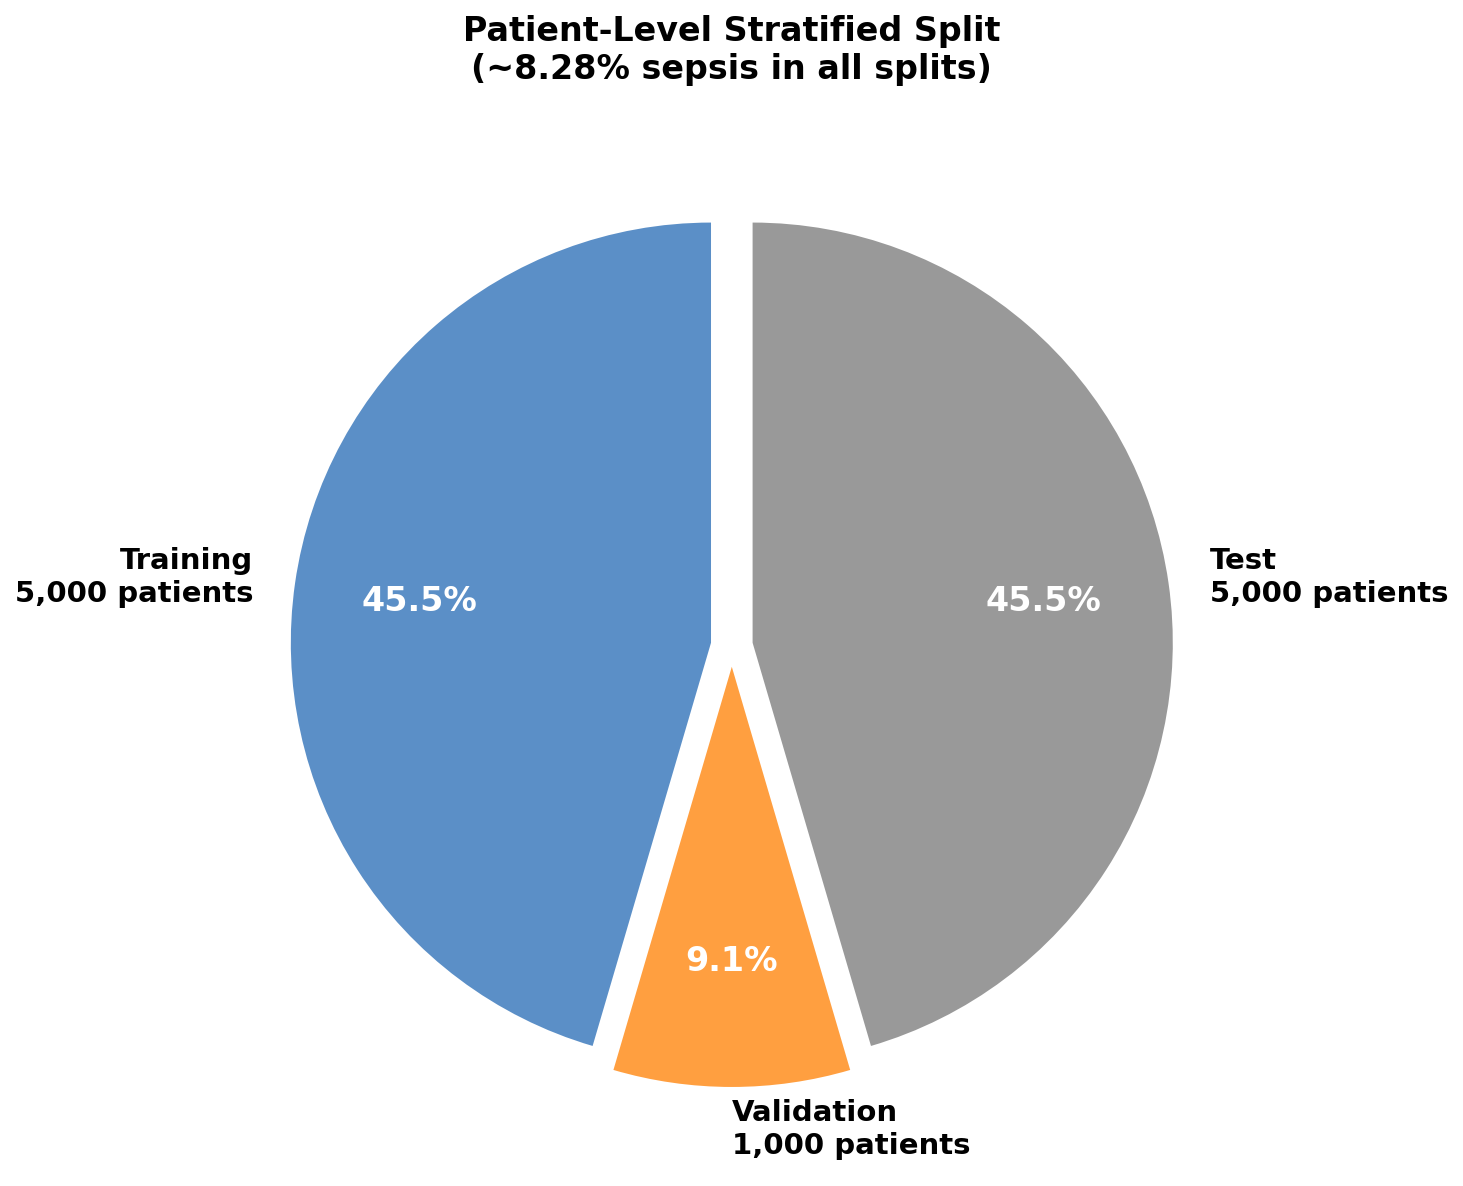
\includegraphics[width=0.38\textwidth]{chart1_split.png}
\caption{Patient-level stratified split showing the distribution of patients across training, validation, and test sets. All splits maintain approximately 8.28\% sepsis prevalence, reflecting the severe class imbalance characteristic of real-world clinical data.}
\label{fig:dataset_splits}
\end{figure}
\FloatBarrier

\begin{figure}[htbp]
\centering
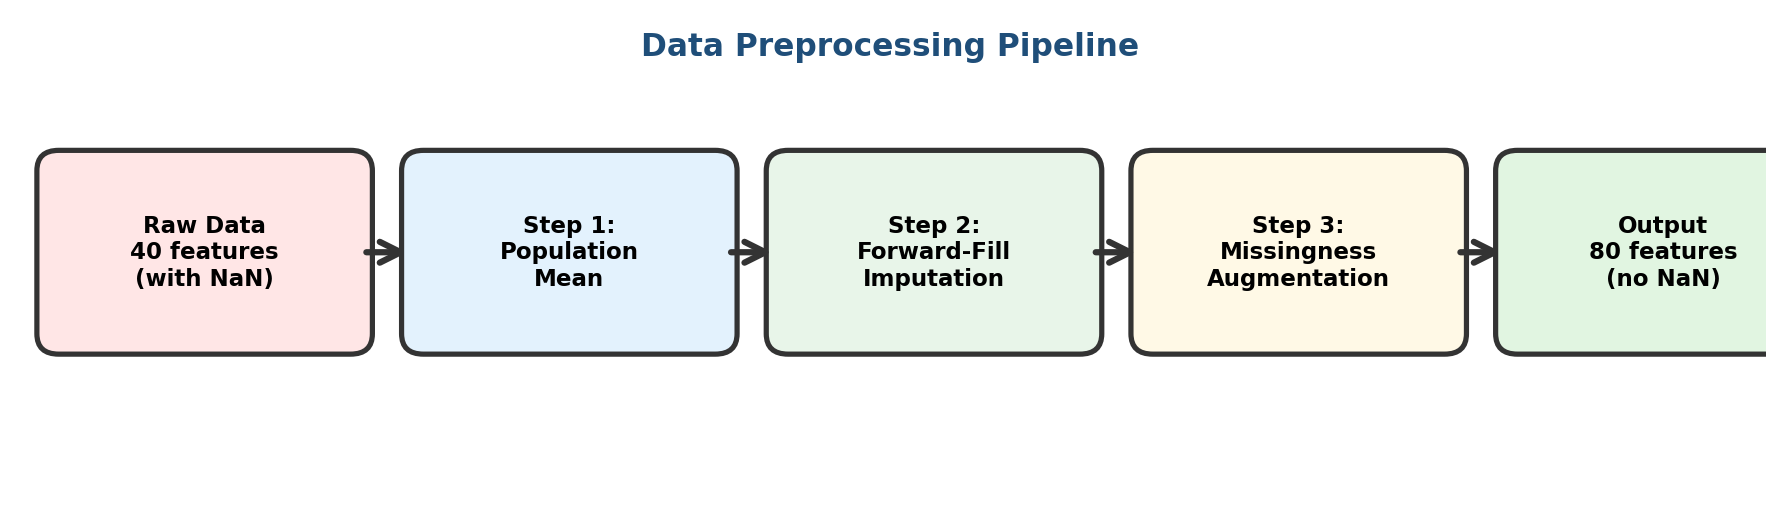
\includegraphics[width=0.5\textwidth]{chart3_pipeline.png}
\caption{Data preprocessing pipeline from raw data to model-ready features. The pipeline consists of population mean computation, forward-fill imputation, and missingness augmentation, transforming the raw 40-feature input into an 80-dimensional feature space suitable for training.}
\label{fig:preprocessing_pipeline}
\end{figure}
\FloatBarrier

\begin{figure}[htbp]
\centering
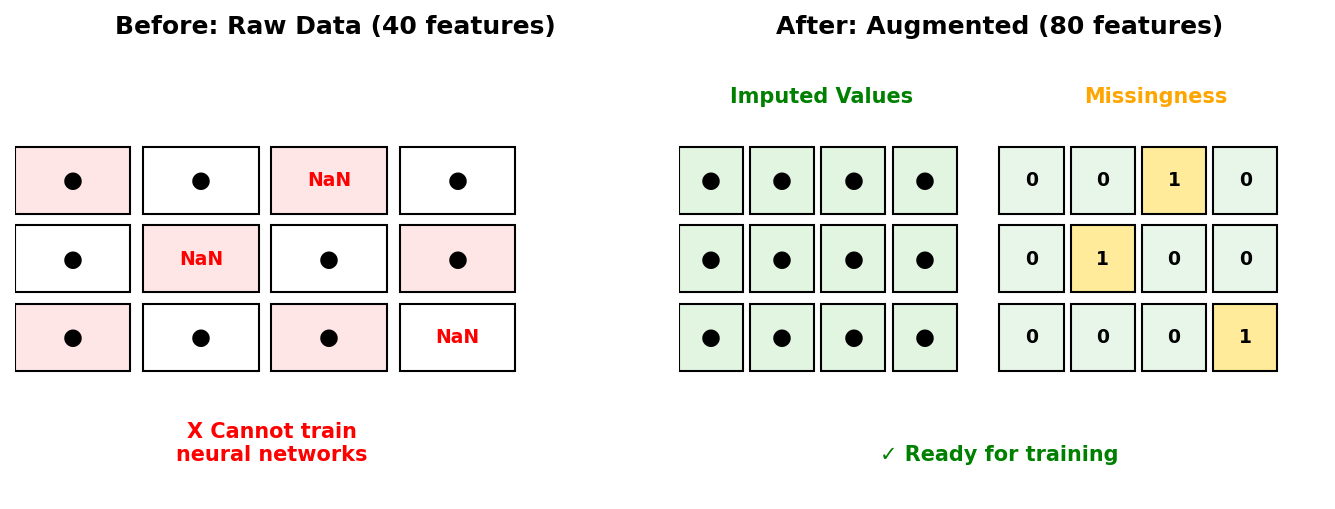
\includegraphics[width=0.5\textwidth]{chart5_transformation.png}
\caption{Feature transformation showing how raw data with missing values (NaN) is converted into training-ready format. The left panel shows the original 40 features with missing values that cannot be processed by neural networks. The right panel shows the augmented 80-feature representation with imputed values (green) and corresponding missingness indicators (orange), preserving information about which values were originally missing.}
\label{fig:feature_transformation}
\end{figure}

\subsection{Approach 1: Autoencoder + k-NN}

Our first approach involves using an autoencoder to train a feature embedding of each data point, followed by a k-NN clustering algorithm on individual data point representations to classify new data points.

The motivation behind using an autoencoder is that we have a large number of complex features. In addition to the 40 initial biomarkers and 40 missingness labels, we included 80 additional augmented features to capture relevant temporal information. These temporal features were an exponential moving average of the previous 7 data points and a simple linear difference from the previous data point for each of the 40 biomarkers.

With such a complex system, we decided to train an encoder by extracting the first half of an undercomplete autoencoder to reduce dimensionality and learn a theoretically more useful disease representation that captures the relevant signal from noise. We found that autoencoder with two hidden encoding layers, a 32-dimension embedding layer, and two hidden decoding layers worked best for this task. We additionally used ReLU for nonlinearilty and dropout ($p=0.5$) during training to prevent overfitting. We used the Adam optimizer and mean-squared error as the reconstruction loss.

\begin{figure}[htbp]
\centering
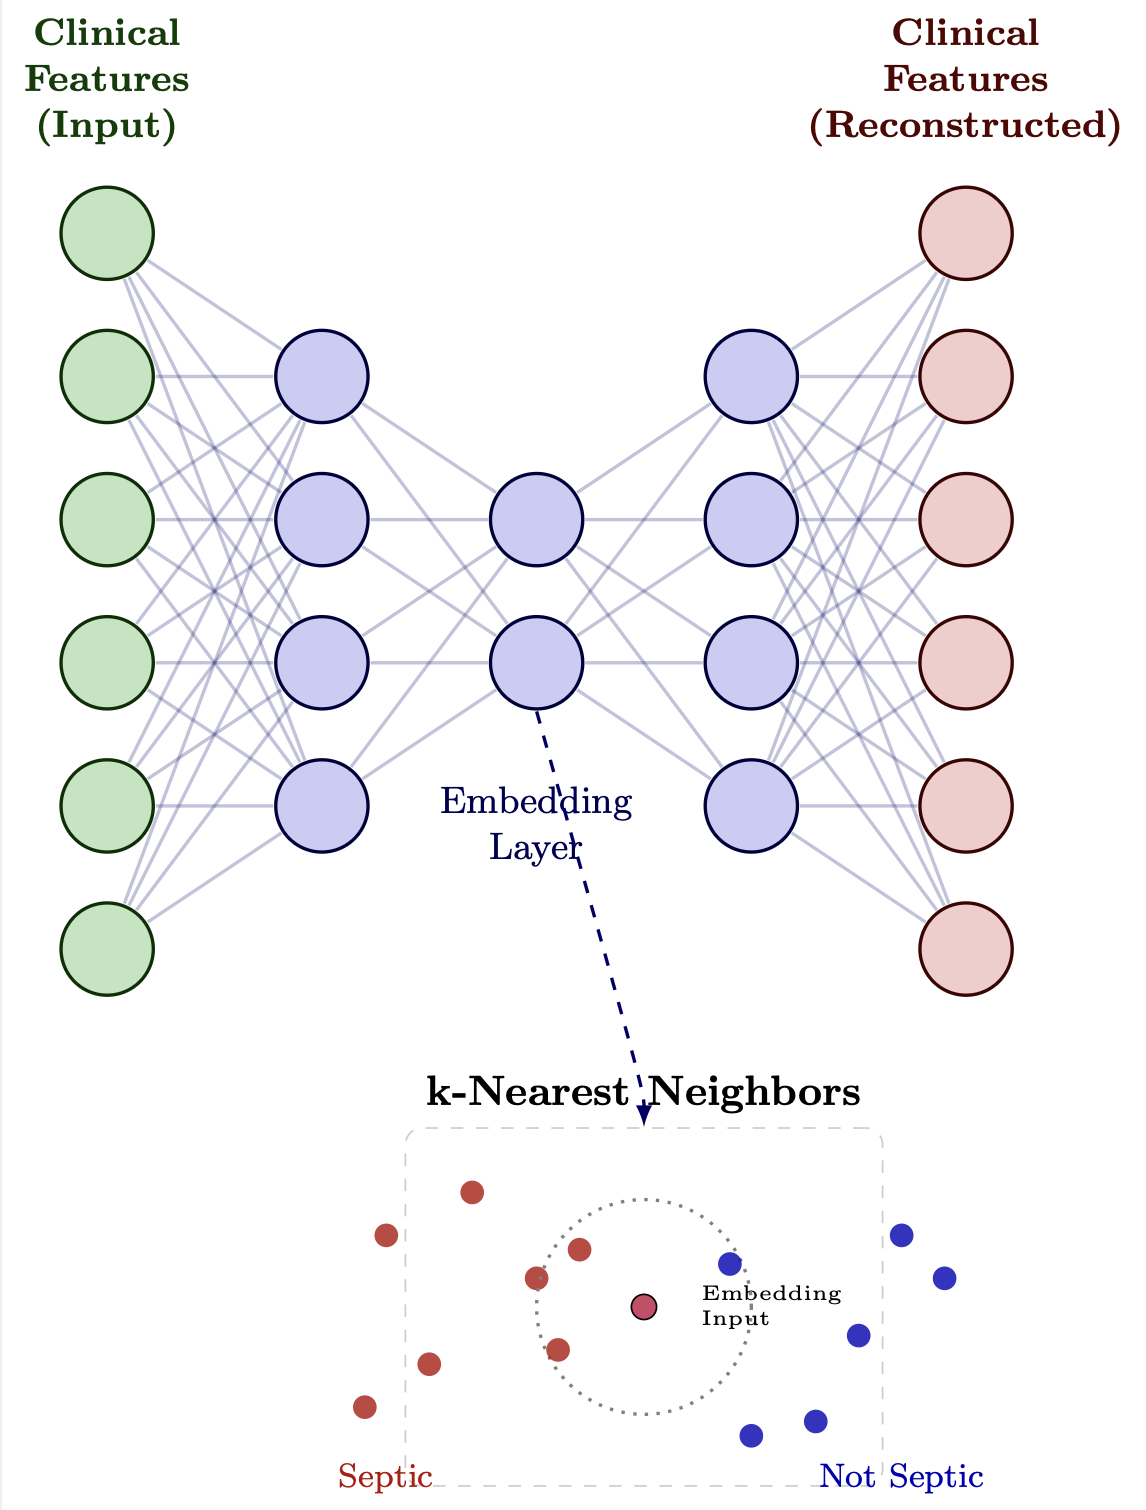
\includegraphics[width=0.4\textwidth]{autoencoder_knn_arch.png}
\caption{Autoencoder + k-NN Architecture}
\label{fig:autoencoder_knn_arch}
\end{figure}

Applying a clustering algorithm provides several benefits from a clinical and interpretability perspective. Clustering algorithms can often discover hidden structure within a dataset. This is especially valuable in the context of sepsis detection, since sepsis can often present in many different ways. A clustering algorithm might be able to identify subtypes and phenotypes that would additionally assist a clinical professional in providing targeted treatment conditions. Using manual tuning, we found that $100$ nearest neighbors resulted in the best predictive performance in the validation set. 

Although KNN does not have a tunable threshold like the other classification models, we attempted to address class imbalance by combining two different reweighting methods. First, we gave datapoints in the minority class greater per-datapoint weighting proportionally to their rarity. This ensures that the total "voting power" is the same across classes. A single minority class datapoint is now able to counteract multiple majority class datapoints in voting, which has the same effect as lowering the threshold for the minority class, even though KNNs do not have an explicit probability threshold. We will refer to the unbalanced weighting as naive and the rebalanced weighting as balanced.

Additionally, we did inverse distance reweighting, such that closer datapoints are weighted more than farther datapoints in proportion to the inverse distance. This accounts for the phenomena of a extreme majority class often being considered for voting--even when it isn't in the same cluster--due to the much higher prevalence of the majority class overall.

\[w_{dist}=\frac{1}{\text{distance}+\epsilon}\]

Thus, the final calculation for the probability of a data point belonging to each sepsis class is as follows:

\[\text{Sepsis score} = \sum_{i \in \text{neighbors}} (w_{dist}^{(i)} \cdot w_{class}^{(label_i)} \cdot \mathbb{I}(label_i = \text{sepsis}))\]


\subsection{Approach 2: Transformer Model}

Clinical time-series data incorporates complex, long-range physiological relationships, like blood pressure trends, oxygen saturation, and lab results, which influence one another across time. This makes it challenging for rule-based methods or single-step models to capture disease progression effectively. Transformers are well-suited for this domain because they model global temporal dependencies through self-attention.

For this task, we use an encoder-only Transformer \cite{vaswani2017attention}. As this task is per-time-step sequence labeling, at each hour, we estimate the real-time probability that a patient will develop sepsis in the near future. Unlike encoder-decoder architectures used for sequence generation, our Transformer encoder produces a hidden state for each timestep, preserving the temporal structure of clinical trajectories. Further, with input dimensionality reduction, we maintain lightweight size to improve the speed of clinical prediction. For physiological, data-based, and practical concerns, the Transformer model paired with dimensionality reduction is thus a solid choice.

\begin{figure}[htbp]
\centering
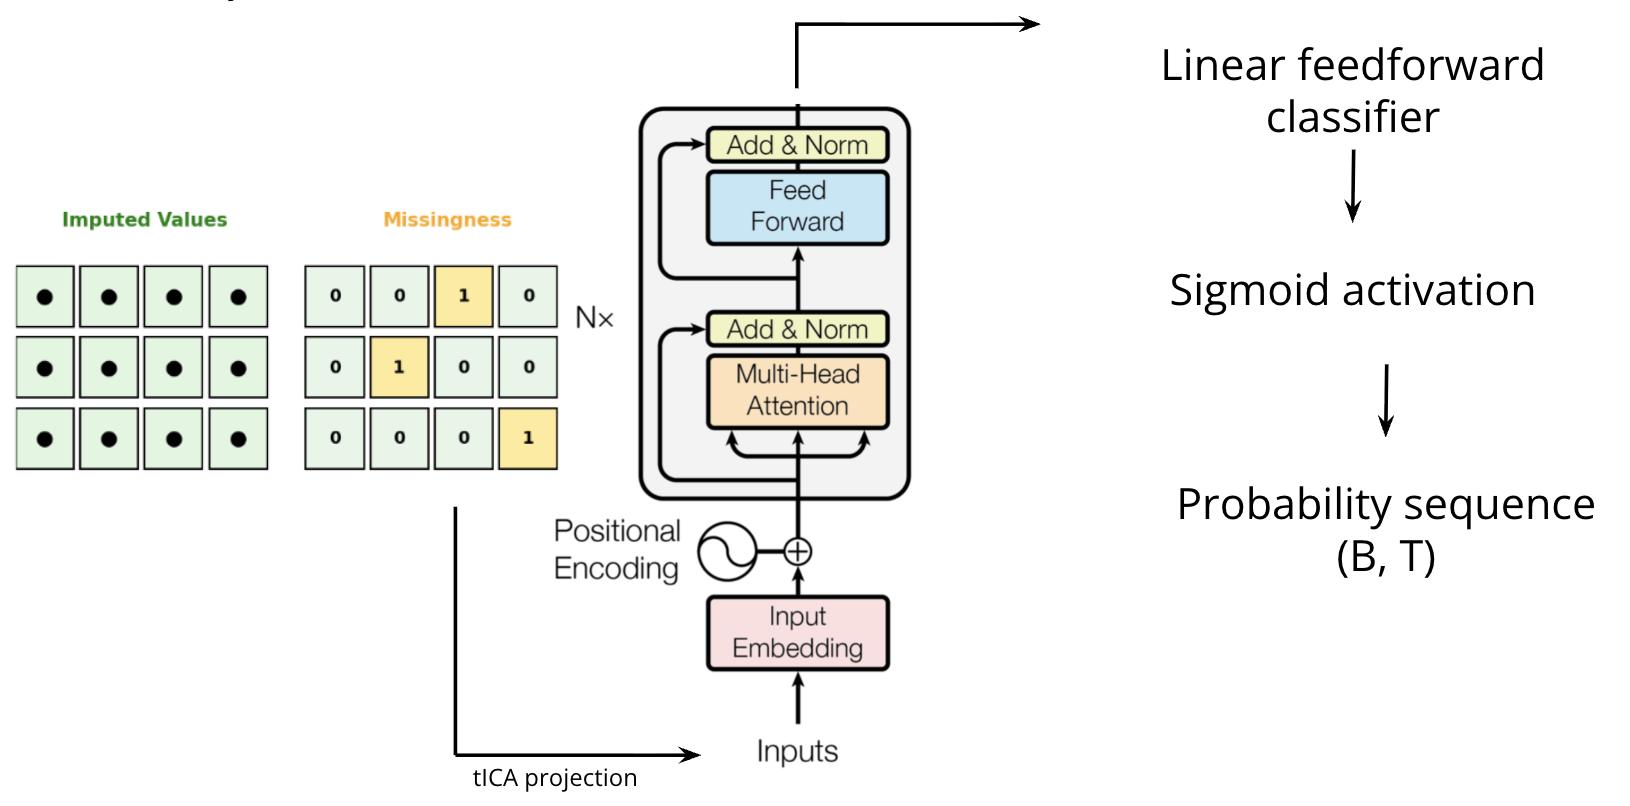
\includegraphics[width=0.48\textwidth]{Transformer_Fig1.png}
\caption{Transformer Model Architecture and Formulation}
\label{fig:transformer_fig1}
\end{figure}

The data is initially composed of physiological data from time-series in 40 normalized clinical variables. For hours where no data is yet observed, we fill values using a population mean and include a missingness mask, allowing the model to distinguish between truly normal readings and unmeasured signals. The input is reduced through time-lagged independent component analysis (tICA) projection to remove redundant correlations and improve stability. Positional encodings maintain ordering of events over time.

tICA is known to be effective for time-series data and has gained popularity in analyzing molecular dynamics trajectories. Since it incorporates traces of previous timesteps in future timesteps, its analysis can be helpful. However, the difference from ICA was small. Further, an increase in tICA lag (carryover from previous time steps) did not noticeably improve performance.

Then, a lightweight N-layer Transformer encoder (N = 2 or 3) applies multi-head self-attention, feedforward layers, and residual + LayerNorm blocks to model complex physiological interactions across long time horizons. A linear classifier then maps each timestep’s hidden state to a raw risk score, followed by a sigmoid to obtain a probability sequence in the form of logits (B, T).

Hyperparameter tuning is performed using Bayesian Optimization (Optuna). We treat model design as an unknown landscape where each point is a specific set of hyperparameters (e.g., component analysis dimension, number of heads, dropout, embedding size, learning rate). After each trial, the surrogate model is updated using the observed performance, allowing the optimizer to balance exploration and exploitation. As more trials are completed, the best achievable utility improves and eventually plateaus, revealing an optimal operational model under clinical constraints.

\begin{figure}[H]
\centering
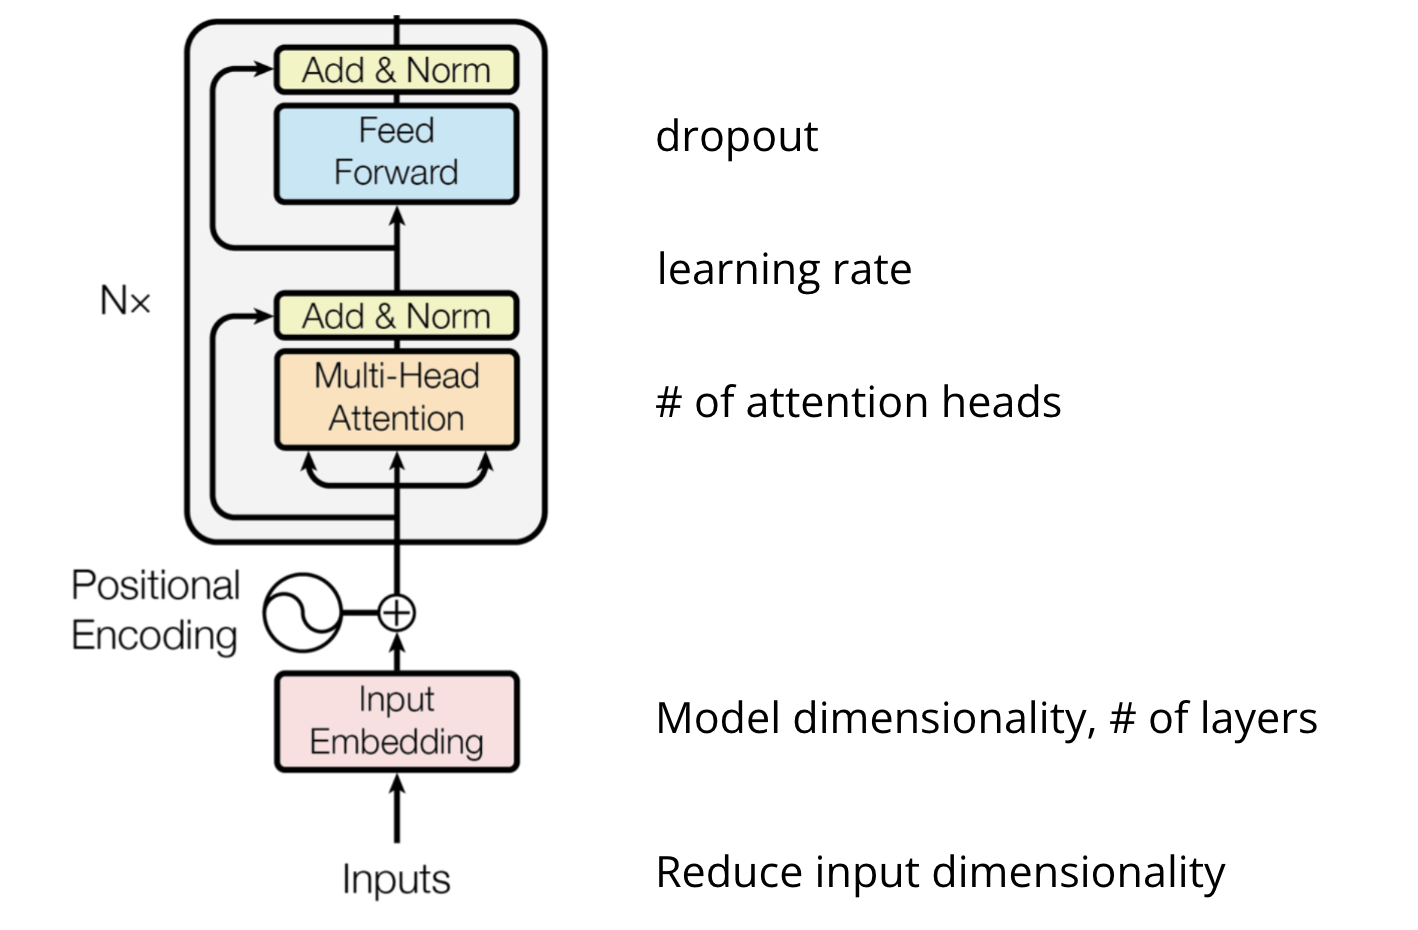
\includegraphics[width=0.48\textwidth]{Transformer_Fig2.png}
\caption{Transformer Model Architecture Parameters} 
\label{fig:transformer_fig2}
\end{figure}

The transformer model was trained using binary cross-entropy loss and early stopping to reduce the extent of overfitting, with patience of 5 and a maximum of 20 epochs.

\subsection{Approach 3: LSTM Model}

LSTMs are well-suited for handling long-range relationships in time series data. Like transformers, they are good at capturing trends over long periods of time, and are robust to vanishing/exploding gradients that other RNNs may face when dealing with long sequences. Robustness against long sequences is important for real-life clinical scenarios, where patient data can be collected for long periods of time prior to the onset of symptoms.

In the context of the PhysioNet Challenge, LSTMs perform well for early predictions of diagnoses since LSTM processes sequences causally, one timestamp at a time. For example, a patient who currently has metrics that would be considered normal may still be flagged by LSTMs analyzing the trend up to that point. In a clinical context, early flags like these do not need to immediately lead to diagnoses to  provide utility. Early alerts can help additional tests to be run and protective measures to be taken preemptively. 

For each patient and hour $t$, a 80-dimensional feature vector including 40 normalized clinical variables and 40 missingness indicators. To account for variation across patient time series, we batched them using padded sequences. The prediction model is a two-layer LSTM, each with 128 hidden units and a dropout rate of 0.3. We have a unidirectional LSTM because we are interested in modeling causally. The output is softmax, which maps probability of sepsis at each hour. 

\begin{figure}[H]
\centering
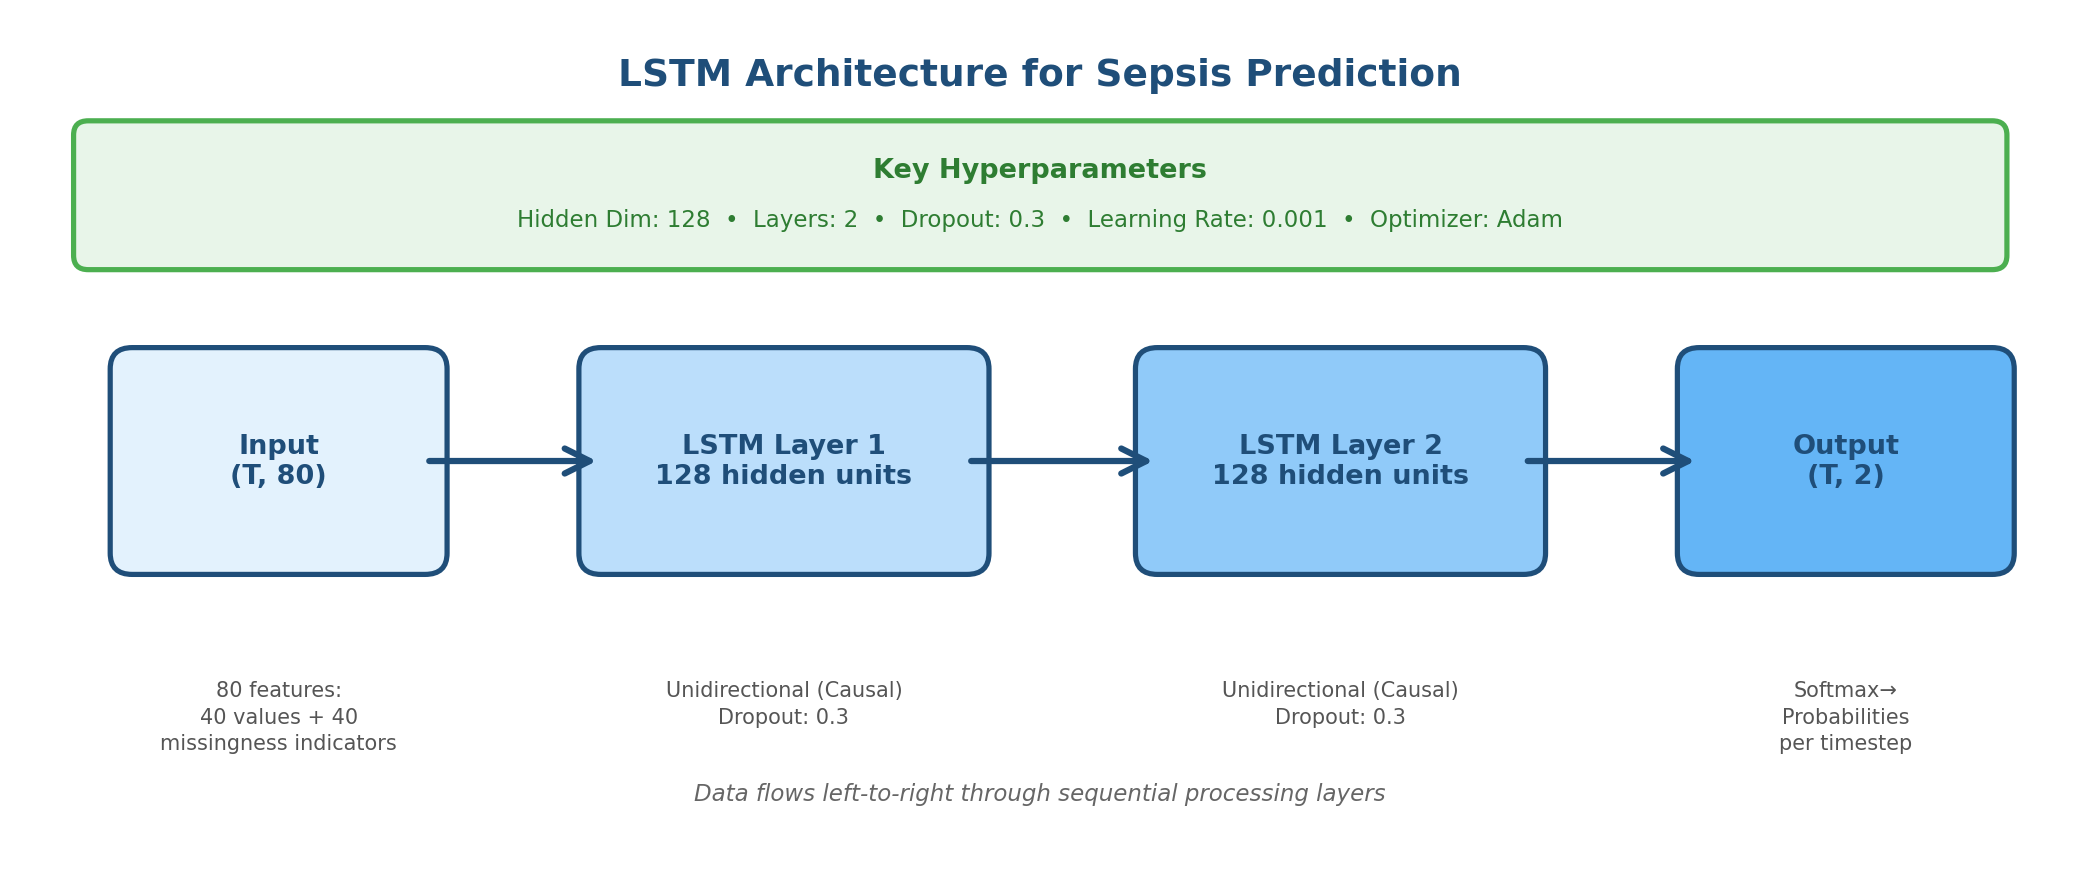
\includegraphics[width=0.48\textwidth]{chart6_lstm_architecture.png}
\caption{LSTM architecture for sepsis prediction. The model consists of two stacked LSTM layers with 128 hidden units each, processing
80-dimensional input features (40 clinical values plus 40 missingness indicators) in a unidirectional manner to preserve causal ordering. Dropout
of 0.3 is applied between layers to prevent overfitting. The output layer uses softmax activation to produce per-timestep probability estimates
for sepsis risk.}
\label{fig:lstm_architecture}
\end{figure}

The model was trained using binary cross-entropy loss with class weights
  inversely proportional to class frequencies to address the severe class
  imbalance. We used the Adam optimizer with a learning rate of 0.001 and
  batch size of 32. Training employed early stopping with patience of 10 epochs
  based on validation utility score, with a maximum of 100 epochs. The dataset
  was split 60/20/20 for training, validation, and testing.

\begin{figure}[htbp]
\centering
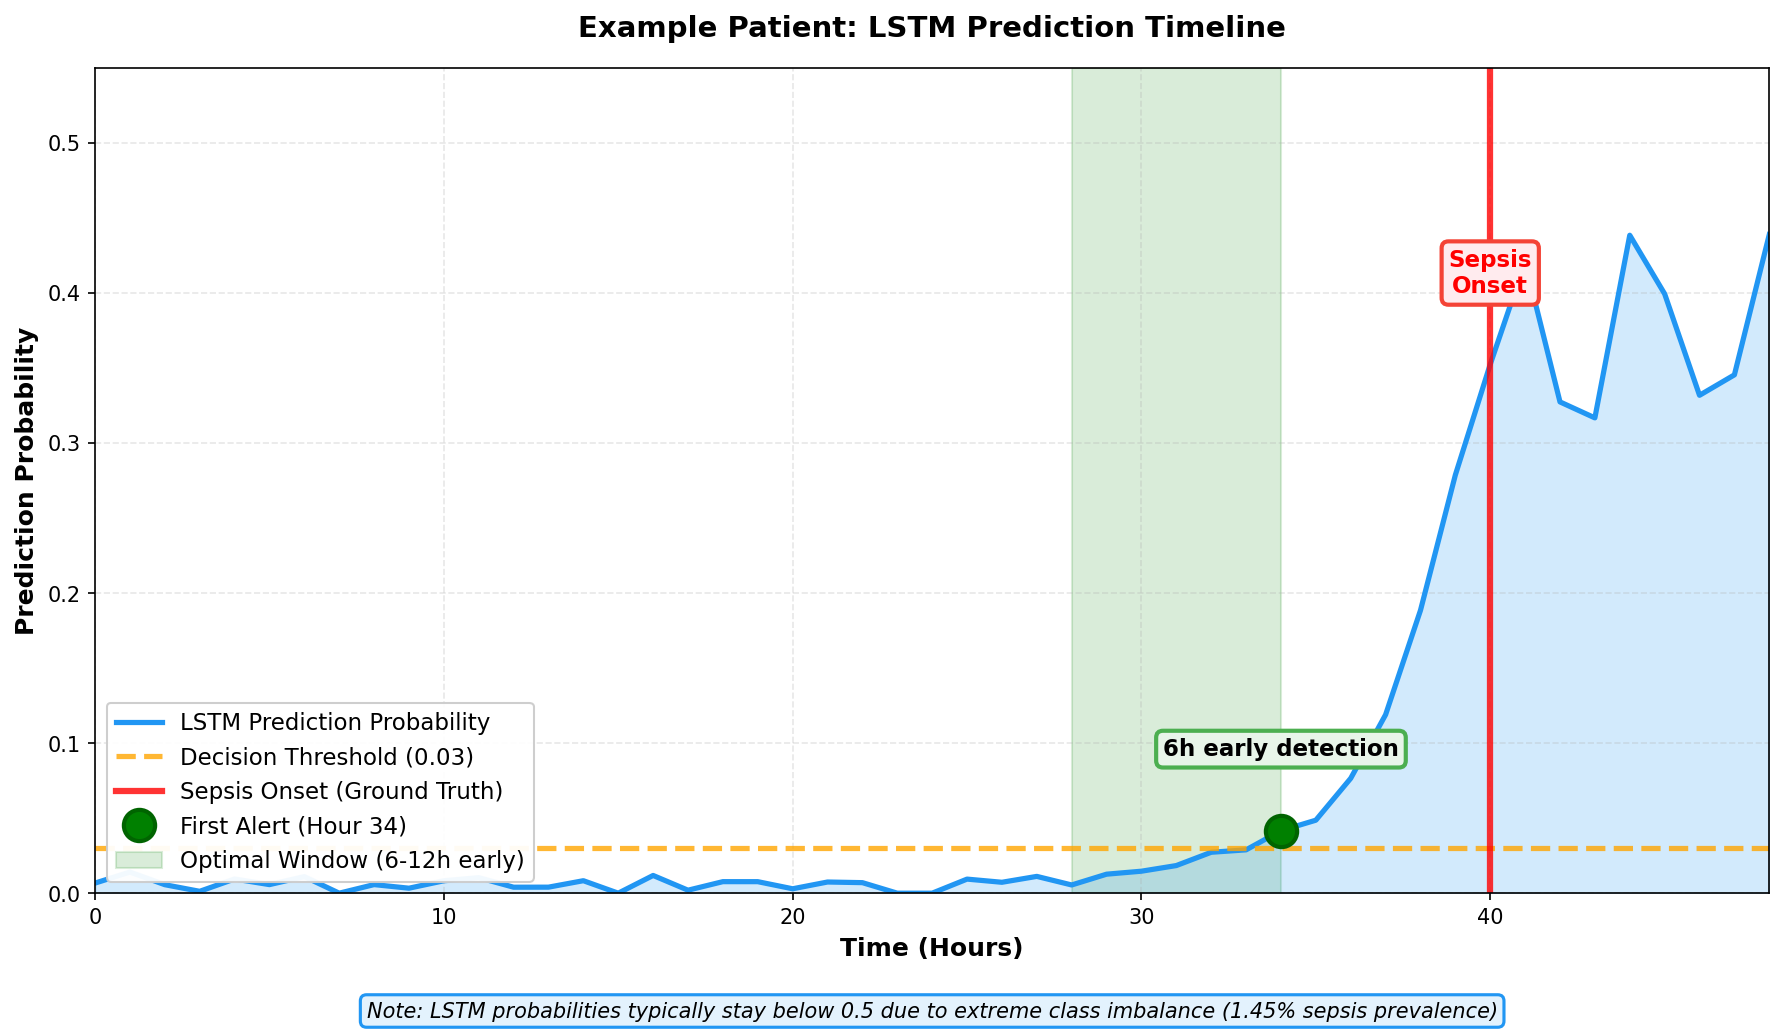
\includegraphics[width=0.45\textwidth]{chart9_prediction_timeline.png}
\caption{Example patient prediction timeline demonstrating the LSTM's causal, sequential processing. The model begins with low sepsis probability
predictions and gradually increases risk assessment as it processes incoming hourly measurements. In this case, the model crosses the decision
threshold (0.03) at hour 34, providing a 6-hour early warning before actual sepsis onset at hour 40. This illustrates how the LSTM can flag
patients based on temporal trends even when current vital signs appear normal, enabling clinically actionable early alerts.}
\label{fig:lstm_prediction_example}
\end{figure}
\FloatBarrier

\subsection{Utility Function}
The utility function used to evaluate the sepsis prediction model is designed to reward meaningfully-timed alerts while penalizing harmful or unnecessary alarm behavior. For patients who develop sepsis, the model gains positive utility when it alerts early enough to influence treatment. It gradually increases from zero to full reward when alerts occur 12–6 hours before onset and reaches maximum benefit in the optimal 6–0 hour window prior to sepsis. Late or missed detections, specifically between 6 hours before to 3 hours after onset, have increasing penalties as delayed recognition can lead to worse outcomes. 

\begin{figure}
\centering
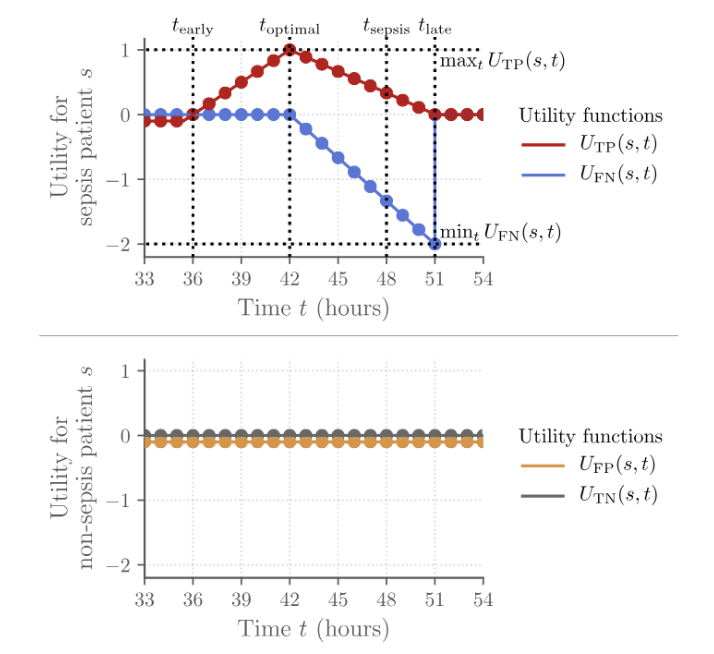
\includegraphics[width=0.5\textwidth]{Utility_Fig2.png}
\caption{Utility functions for true positive utility (red), false negative utility (blue), false positive utility (orange), and true negative utility (black).}
\label{fig:utility_fig2}
\end{figure}

For non-sepsis patients, false alarms accumulate a small negative utility per timestep to discourage excessive alerting that can contribute to alarm fatigue, while true negatives remain neutral. Utility is summed across all time steps to generate a per-patient score that fairly accounts for different lengths of stay. Lastly, the total model utility across all patients is normalized to a 0–100\% scale using the performance of a perfect model and a no-alert baseline as anchors, producing an interpretable metric. Thus, this score captures correctness and timeliness, aligning model evaluation with real-world clinical output. 

\begin{figure}[H]
\centering
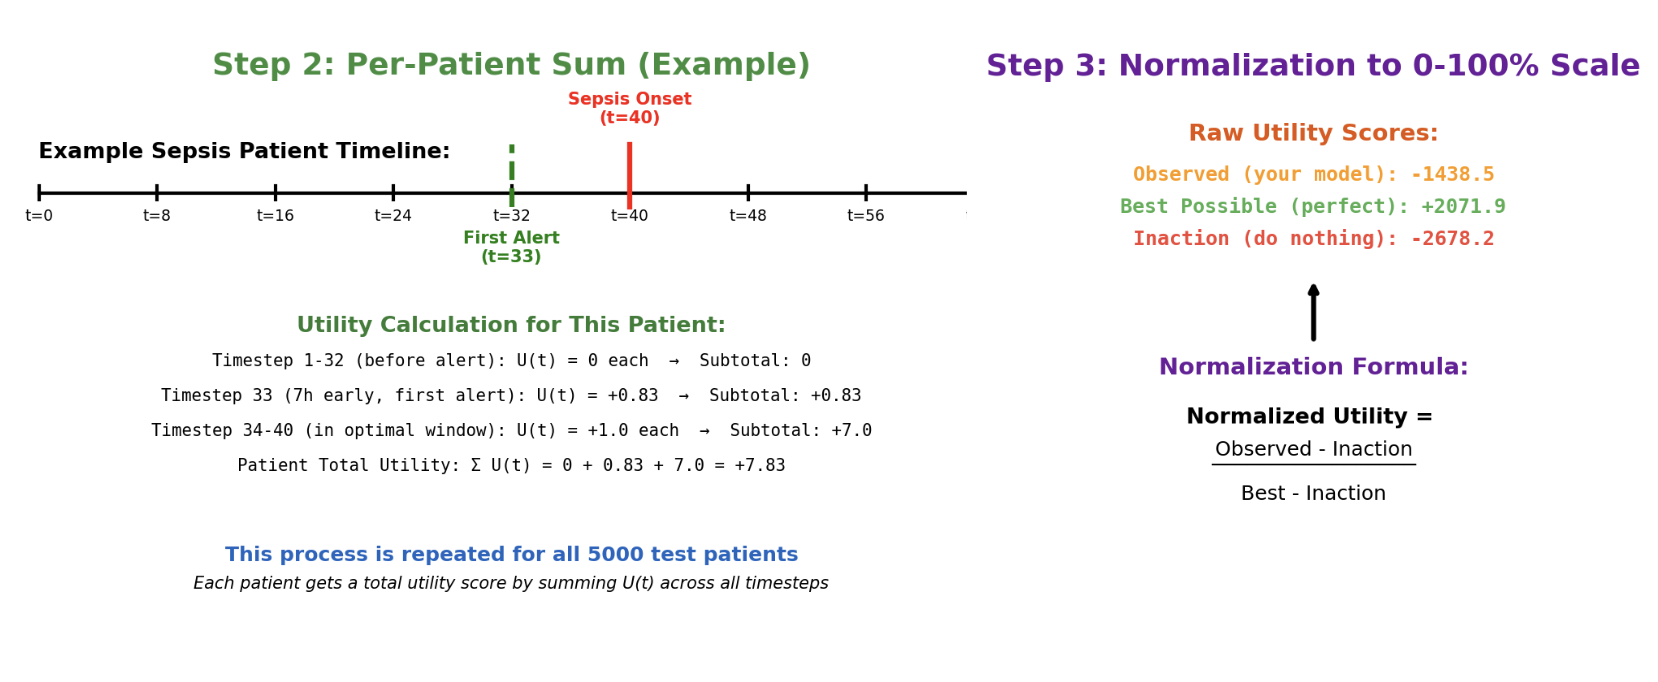
\includegraphics[width=0.5\textwidth]{Utility_Fig1.png}
\caption{Example utility function calculation. }
\label{fig:utility_fig1}
\end{figure}

\section{Results}

\subsection{Logistic Regression Baseline}
After optimizing the alert threshold (=0.03), the model achieved a test utility score of 0.10, with AUC = 0.60 and AUPRC = 0.03. While these results demonstrate that missingness alone provides a very weak but non-zero sepsis signal, the model treats each timestep independently and fails to capture any temporal trends or physiological dynamics. The logistic model performed reasonably but did not present with a sufficient fraction of optimal clinical benefit. Overall, this baseline reinforces that simple static models are insufficient for early sepsis prediction and motivates the need for temporal deep learning architectures.

\subsection{Autoencoder + k-NN}

An AUROC of 0.651 and an AUPRC of 0.038 were achieved with time augmented features and class reweighting, achieving a utility of 0.04. This is the only "failure" of our three models in that the overall performance was worse than the baseline logistic regression. 

\begin{figure}[H]
\centering
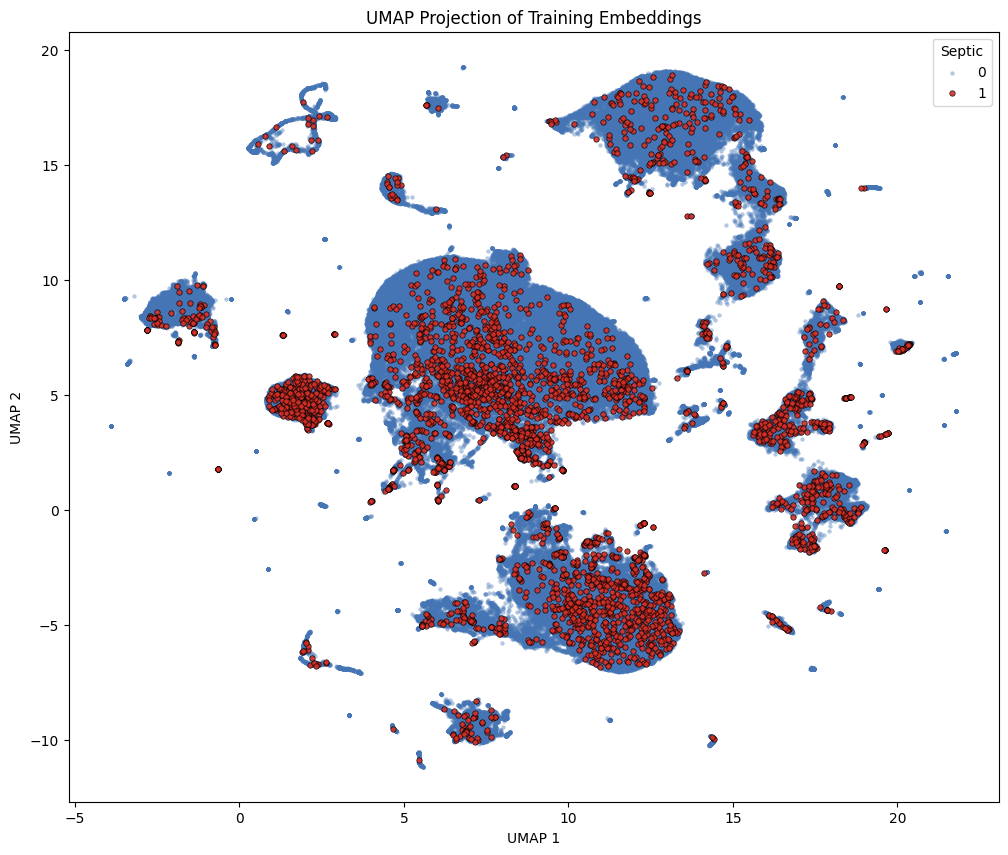
\includegraphics[width=0.4\textwidth]{Unknown.png}
\caption{UMAP projection of augmented autoencoder embeddings}
\label{fig:UMAP}
\end{figure}

Additionally, we compared the effects of the decision on whether to include time-series data and whether to weight based on class. Including time-series data helped both the AUROC and AUPRC and gave greater definition to the UMAP clusterings (UMAP projection of naive autoencoder not shown). That is, the data points formed clearer clusters with some separation of the septic and non-septic classes. Weighting the septic class more heavily also increased AUROC and AUPRC, though very slightly.

\begin{table}[H]
\centering
\resizebox{\columnwidth}{!}{
\begin{tabular}{|c|c|c|c|c|}
\hline
& \multicolumn{2}{c|}{Class unweighted} & \multicolumn{2}{c|}{Class weighted} \\
\hline
& \textbf{AUROC} & \textbf{AUPRC} & \textbf{AUROC} & \textbf{AUPRC} \\
\hline
\textbf{Naive} & 0.632 & 0.030 & 0.639 & 0.032 \\
\hline
\textbf{Augmented} & 0.649 & 0.037 & 0.651 & 0.038 \\
\hline
\end{tabular}
}
\end{table}

We will now try to understand the various failure modes that might be attributed to this behavior. Sepsis is inherently a trajectory-dependent condition, and meaningful clinical differentiation often hinges on how rapidly biomarkers evolve rather than on their instantaneous values. Our feature engineering pipeline, which relied on handcrafted summaries of each patient’s time series, was unable to fully capture these temporal dynamics. As a result, the clustering algorithms tended to conflate patients who were chronically ill but stable with those who were acutely deteriorating, obscuring clinically important distinctions between “sick but static” and “sick and getting sicker.” This issue was likely compounded by noise introduced during data imputation. Because missingness in clinical records is often informative—patients may not undergo certain tests precisely because clinicians judge them to be relatively stable—replacing missing values with global means can dilute meaningful signal even when missingness indicators are explicitly included. The baseline models were able to exploit the temporal pattern of missingness directly, whereas the autoencoder architecture may have inadvertently blurred or discarded this structure during compression.

These limitations are reflected clearly in the UMAP visualizations, where the latent representations failed to form clinically coherent clusters and sepsis and non-sepsis cases were heavily interleaved. Such overlap suggests that the learned embedding did not encode strong sepsis-specific structure; instead, local neighborhoods were dominated by mixed populations of generally ill patients. This has direct consequences for downstream k-nearest neighbor classification: when nearest neighbors are clinically similar “sick” individuals but not necessarily septic, local majority voting becomes unreliable. Overall, the primary shortcoming of our approach was the lack of learned temporal features or inductive biases capable of modeling disease trajectories. By collapsing rich time-series information into static heuristic features, the model systematically misrepresented severely ill patients as sepsis-positive and obscured the distinctions necessary for accurate clustering and classification.

Finally, as we observe with the other models, threshold selection is extremely important for this classification task because of the nuanced utility function and extreme class imbalance. The attempts described previously in the paper aimed to address this issue with the KNN architecture despite it's lack of an explicit "probability threshold", and we do observe small performance gains in comparison to a naive KNN clustering algorithm. However, we could have potentially improved performance by sweeping through a greater number of reweighting parameters to better optimize the model for our utility function.

\subsection{Transformer}
An AUROC of 0.949 and an AUPRC of 0.355 were achieved. By selecting a threshold of approximately 0.03, the model acquired best utility on the validation set, and its performance on the test set was measured. However, AUROC and AUPRC values are calculated using all timestamps, so utility score is the more relevant metric and for that reason only the utility graph for the validation set is included below. While a utility score of 0.578 was obtained, it should be noted that many false positives occurred.

\begin{figure}[H]
\centering
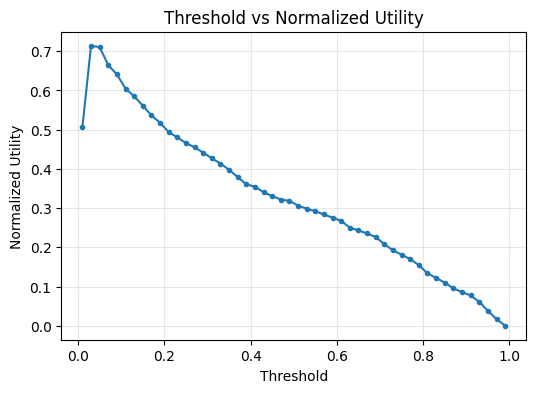
\includegraphics[width=0.44\textwidth]{threshold.png}
\caption{Transformer Model Threshold Determination using Utility Function on Validation Set} 
\label{fig:transformer_R1}
\end{figure}

Lead times for sepsis patients show at what time steps the model predicted the patient to be septic. Further, a bar graph is provided to better understand the bucketing of model prediction times and rates of correct prediction. While nearly half of sepsis patients were predicted optimally and nearly four-fifths predicted on time or earlier, the false alarm rate was fifty percent. Unfortunately, this means that the model is not specific enough and requires human-assisted judgment. The transformer is not very explainable, but it is likely that component analysis played a large part in improving performance.

\begin{figure}[H]
\centering
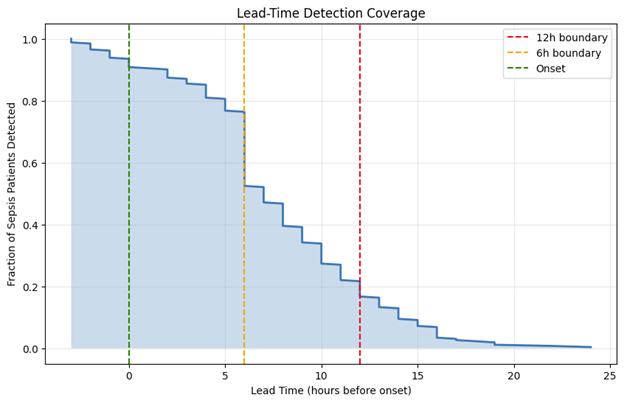
\includegraphics[width=0.5\textwidth]{lead_times.png}
\caption{Transformer Model Patient-Level Lead Times} 
\label{fig:transformer_R2}
\end{figure}

\begin{figure}[H]
\centering
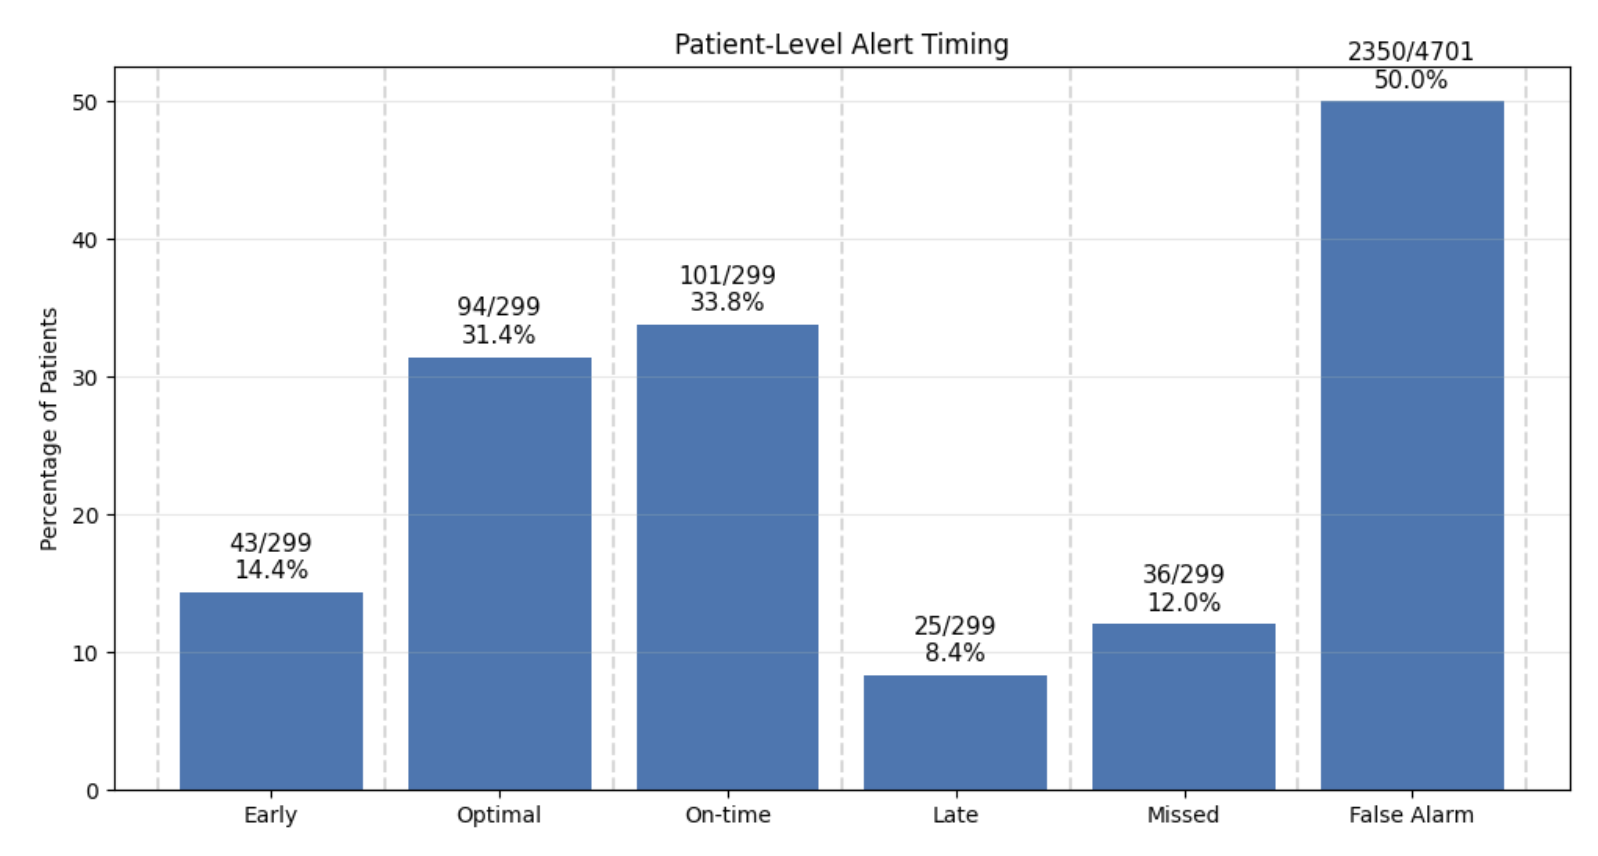
\includegraphics[width=0.5\textwidth]{Transformer_R2.png}
\caption{Transformer Model Patient-Level Alert Timing} 
\label{fig:transformer_R2}
\end{figure}

\subsection{LSTM}
The LSTM achieved an AUROC of 0.737 and an AUPRC of 0.051. An AUROC of 0.737 indicates that the LSTM was able to reasonably discriminate between positive and negative sepsis timestamps, consistently assigning higher risk scores to sepsis-positive labels. While an AUPRC of 0.051 appears extremely low, it is consistent with the strong class imbalance of the dataset. The prevalence of sepsis patients in the dataset is only around 8\%, which translates to an even lower fraction of non-septic timestamps. 

However, these metrics are not able to capture meaningful temporal information of individual patient trajectories, since AUROC and AUPRC are computed over all timestamps pooled together. Furthermore, given the nature of the task where early predictions are required, a high number of false positive timestamp labels are expected. For this reason, the utility score is a better metric that directly encodes the clinical preferences where detecting sepsis within a relevant time window is critical.

The optimal threshold was identified as 0.03 based on the threshold-utility curve. The model achieved a validation utility of 0.272 and a test utility of 0.261, meaning the model realized around 26\% of the ideal clinical benefit. 

To quantify the timeliness of detection, lead-time detection curves were plotted. Based on this analysis, 36.8\% of all sepsis patients
in the test set received early detection.

\begin{figure}[htbp]
\centering
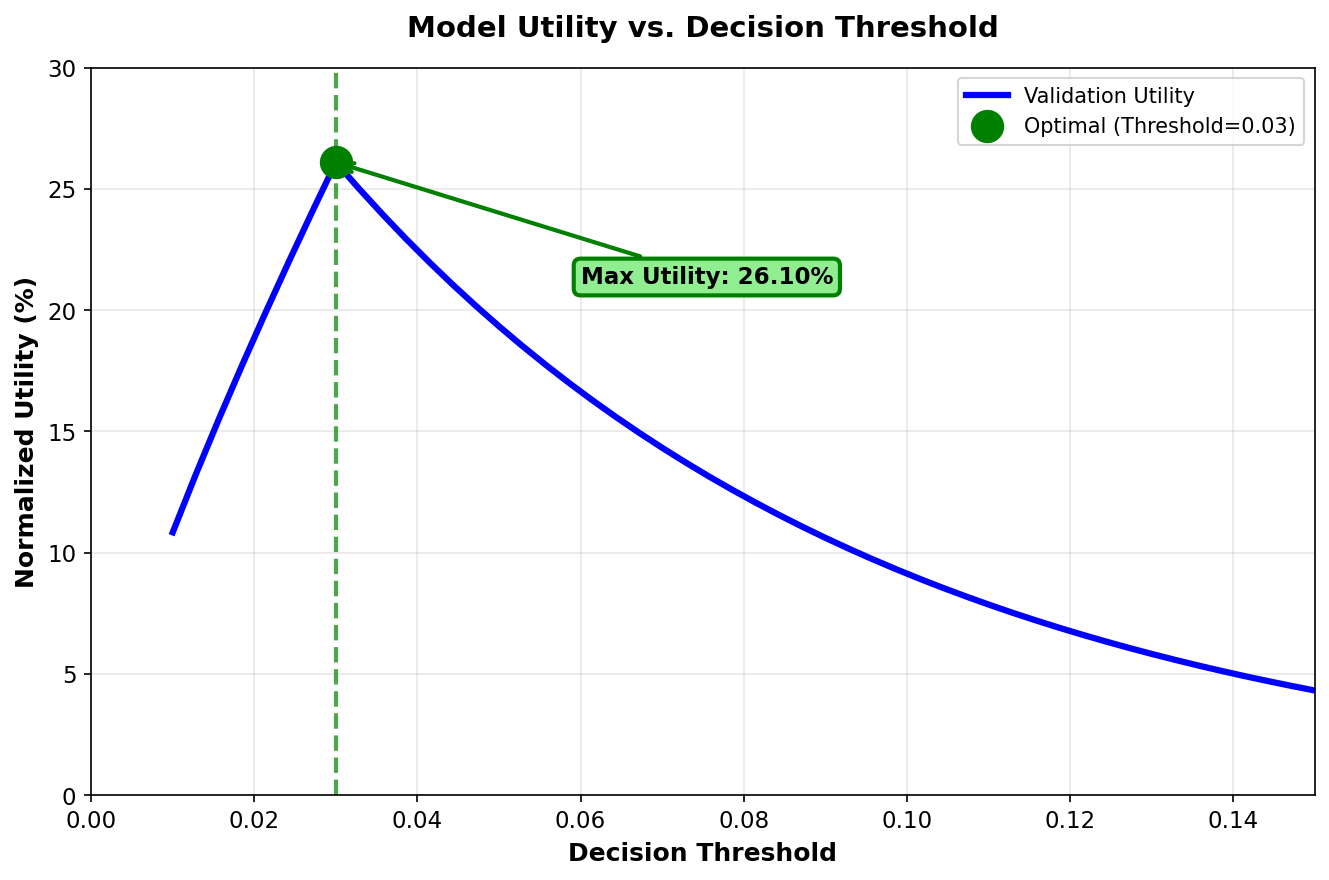
\includegraphics[width=0.5\textwidth]{chart15_utility_threshold.png}
\caption{Normalized utility as a function of decision threshold on the validation set. The optimal threshold of 0.03 achieves maximum utility of
26.10\%, balancing early detection of sepsis cases against false alarm rate. The curve demonstrates the trade-off between sensitivity and
specificity, with utility declining sharply at both very low thresholds (excessive false alarms) and high thresholds (missed detections).}
\label{fig:lstm_utility_threshold}
\end{figure}

\begin{figure}[htbp]
\centering
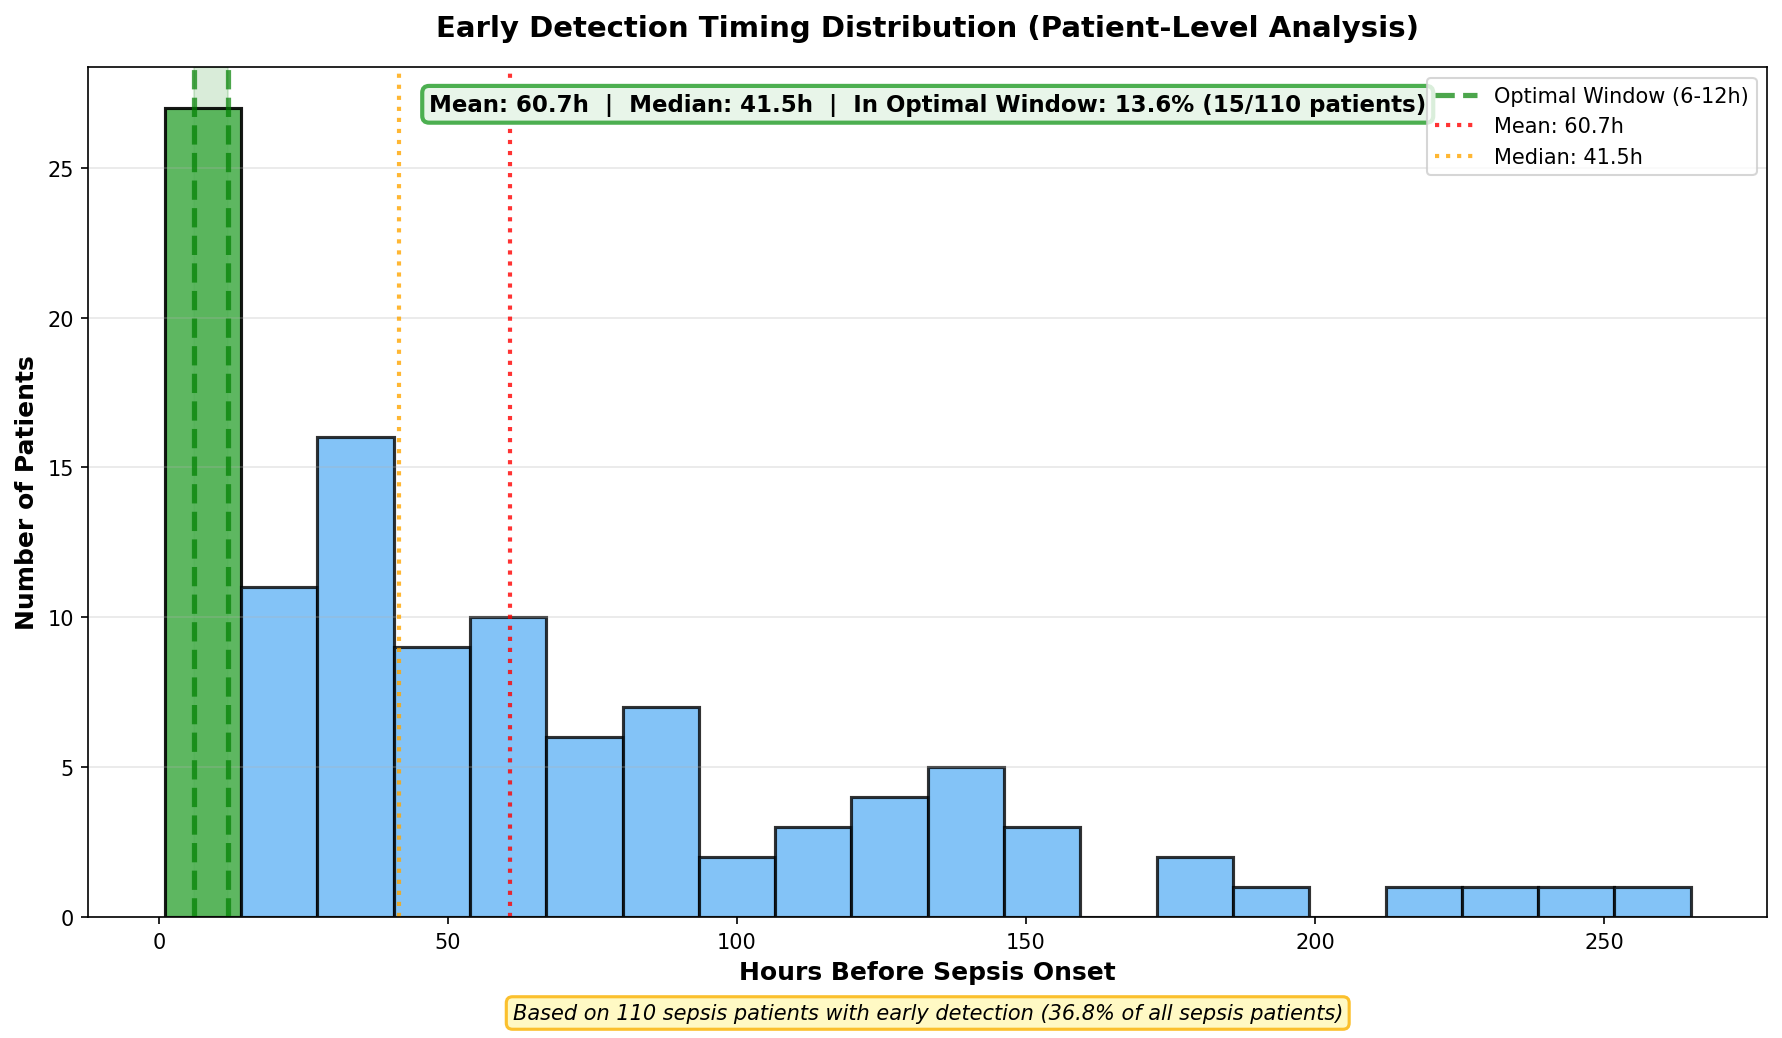
\includegraphics[width=0.5\textwidth]{chart16_early_detection_timing.png}
\caption{Distribution of early detection timing for sepsis patients who were successfully predicted before onset. The histogram shows lead times
ranging from 0 to over 250 hours before sepsis onset, with a mean of 60.7 hours and median of 41.5 hours. The green shaded region (0-12h before
onset) represents the optimal detection window, containing 13.6\% of detected cases (15 of 110 patients). Overall, 36.8\% of all sepsis patients
in the test set (110 of 299) received early detection, demonstrating the model's capability for clinically actionable early warning.}
\label{fig:lstm_early_detection}
\end{figure}


\section{Discussion}

Our results provide some insight into modeling early sepsis prediction. The clinical time-series data is irregular, sparse, and with a large class imbalance that is unique when combined with the nature of how clinical benefit can result from sepsis prediction.

The relative performance of the models is perhaps due to both the nature of the data and the structure of the models. Each model has its own rationale that suggested it could be useful for early sepsis prediction, although some proved to be more useful or robust. To start, the logistic regression baseline reinforces the notion that patterns themselves can be somewhat informative through missingness indicators, but its inability to model trajectories and sufficient complexity severely limits its clinical utility.

The autoencoder–kNN approach did not perform very well, which could have been due to how clustering encoded chronic but stable illness similarly to deterioration in sepsis. Both noise and time-series summaries led to ineffective temporal encoding which likely interfered with discriminative ability even if sliding window aggregations over time were added as a feature. Moreover, the extreme class imbalance could lead neighborhoods to become dominated by non-septic patients, even with reweighting strategies. Thus, embeddings did not have effective separation.

In contrast, the LSTM achieved respectable performance, with gradual physiological changes allowing for early warnings where more than one-third of septic patients received early detection. The structure of the LSTM allows it to be robust in time-series data prediction and this is reflected in its balance of early detection with false alarms.

However, the transformer achieved the strongest performance. An ability to model long-range dependencies and temporal patterns likely allowed it to be more sensitive to sepsis patients and detect potential for sepsis earlier. However, it also predicted roughly half of non-sepsis patients to be at risk, demonstrating low specificity. This poses a burden given the extremely high false positive rate.

A high false positive rate is caused primarily by the large imbalance in the utility function penalties as missing a sepsis case carries a $-2$ penalty, whereas a false positive incurs only $-0.05$ per timestep, which is a 40× difference. As a result, even well-performing models tend to trigger alerts aggressively, which reflects in extremely low optimal decision thresholds such as 0.03 for the LSTM, where a predicted “probability” of just 3\% is enough to raise a red flag. While this behavior may be undesirable at first glance, it aligns with clinical priorities in which early detection is far more valuable than delayed treatment.

Going further, these models can operate within a workflow that combines automated prescreening with manual validation of alerts. This could allow clinicians to disregard false positives while benefiting from timely warnings on high-risk patients. In real-world deployment, the thresholds and utility weightings should be tuned based on the optimal domain expertise and empirical hospital data to successfully balance sensitivity, specificity, and staff bandwidth in diverse care environments.

\section{Conclusion}

This work evaluated three modeling approaches using the 2019 PhysioNet Challenge framework in assessing their utility for early sepsis prediction. Overall, the Transformer model achieved the strongest performance (utility = 0.578), followed by the LSTM (0.261), with the autoencoder baseline performing poorly (0.04). These results suggest that models with implicit temporal priors are most effective for early sepsis prediction, as both the Transformer and LSTM architectures inherently capture time-dependent patterns.

We also see that the utility function, particularly the 40× discrepancy between early and late prediction penalties, strongly influences model behavior by skewing predictions toward identifying sepsis events earlier and more frequently. Thus, the reward for optimal detection and penalty for missed detections far outweighs the penalty for false alarms, leading to the observed very low thresholds and aggressive prediction. While this could amplify false positives in some contexts, it may be beneficial in clinical workflows where early intervention outweighs the cost of unnecessary alerts. This would especially be the case if addressing the alarms is not costly or risky.

Overall, these findings highlight both the promise of temporal deep learning models in facilitating sepsis detection and the importance of carefully designing clinical utility functions based on the data and nature of the prediction task at hand.  

\bibliographystyle{icml2024}
\begin{thebibliography}{99}

\bibitem[Beesley \& Lanspa(2015)]{beesley2015neednewdef}
Beesley, S. J., \& Lanspa, M. J.
\newblock Why we need a new definition of sepsis.
\newblock \emph{Annals of Translational Medicine}, 3(19):296, 2015.
\newblock doi: \url{https://doi.org/10.3978/j.issn.2305-5839.2015.11.02}.

\bibitem[Goldberger et~al.(2000)]{goldberger2000physionet}
Goldberger, A. L., Amaral, L. A. N., Glass, L., Hausdorff, J. M., Ivanov, P. C., Mark, R. G., Mietus, J. E., Moody, G. B., Peng, C.-K., \& Stanley, H. E.
\newblock PhysioBank, PhysioToolkit, and PhysioNet: Components of a new research resource for complex physiologic signals.
\newblock \emph{Circulation}, 101(23):e215--e220, 2000.
\newblock RRID: SCR\_007345.

\bibitem[Hurst(2020)]{hurst2020cost}
Hurst, J.
\newblock The cost of sepsis in lives and dollars.
\newblock \emph{bioM{\'e}rieux Connection}, 2020.
\newblock Available at: \url{https://www.biomerieuxconnection.com/2019/09/05/the-cost-of-sepsis-in-lives-and-dollars/}.

\bibitem[Im et~al.(2022)]{im2022timetoantibiotics}
Im, Y., Kang, D., Ko, R., Lee, Y. J., Lim, S. Y., Park, S., Na, S. J., Chung, C. R., Park, M. H., Oh, D. K., Lim, C., Suh, G. Y., Hong, S., Oh, D. K., Suh, G. Y., Jeon, K., Ko, R., Cho, Y., Moon, J. Y., \emph{et al.}
\newblock Time-to-antibiotics and clinical outcomes in patients with sepsis and septic shock: A prospective nationwide multicenter cohort study.
\newblock \emph{Critical Care}, 26(1):19, 2022.
\newblock \url{https://doi.org/10.1186/s13054-021-03883-0}.

\bibitem[Kaukonen et~al.(2015)]{kaukonen2015sirs}
Kaukonen, K.-M., Bailey, M., Pilcher, D., Cooper, D. J., \& Bellomo, R.
\newblock Systemic Inflammatory Response Syndrome Criteria in Defining Severe Sepsis.
\newblock \emph{New England Journal of Medicine}, 372(17):1629--1638, 2015.
\newblock doi: \url{https://doi.org/10.1056/NEJMoa1415236}.

\bibitem[Reyna et~al.(2019)]{reyna2019early}
Reyna, M. A., Josef, C. S., Jeter, R., Shashikumar, S. P., Westover, M. B., Nemati, S., Clifford, G. D., \& Sharma, A.
\newblock Early Prediction of Sepsis From Clinical Data: The PhysioNet/Computing in Cardiology Challenge.
\newblock \emph{Critical Care Medicine}, 48(2):210--217, 2019.
\newblock doi: \url{https://doi.org/10.1097/CCM.0000000000004145}.

\bibitem[Singer et~al.(2016)]{singer2016sepsis3}
Singer, M., Deutschman, C. S., Seymour, C. W., Shankar-Hari, M., Annane, D., Bauer, M., Bellomo, R., Bernard, G. R., Chiche, J. D., Coopersmith, C. M., Hotchkiss, R. S., Levy, M. M., Marshall, J. C., Martin, G. S., Opal, S. M., Rubenfeld, G. D., van der Poll, T., Vincent, J. L., \& Angus, D. C.
\newblock The Third International Consensus Definitions for Sepsis and Septic Shock (Sepsis-3).
\newblock \emph{JAMA}, 315(8):801--810, 2016.
\newblock doi: \url{https://doi.org/10.1001/jama.2016.0287}.

\bibitem[Tarek(2024)]{tarek2024futureforecastinglstm}
Kareim Tarek.
\newblock Future Forecasting Of Time Series using LSTM: A Quick Guide For Business Leaders.
\newblock \emph{Data Science Collective} (Medium), October 6, 2024.
\newblock Available at: \url{https://medium.com/data-science-collective/future-forecasting-of-time-series-using-lstm-a-quick-guide-for-business-leaders-370661c574c9}.

\bibitem[Vaswani et~al.(2017)]{vaswani2017attention}
Vaswani, A., Shazeer, N., Parmar, N., Uszkoreit, J., Jones, L., Gomez, A.~N., Kaiser, Ł., \& Polosukhin, I.
\newblock Attention is all you need.
\newblock \emph{arXiv preprint arXiv:1706.03762}, 2017.
\newblock Available at: \url{https://arxiv.org/abs/1706.03762}.

\end{thebibliography}

\subsection{Graduate requirements}
As discussed in our meeting, we worked on models as graduate-undergraduate student pairs. 

Approach 1 - Autoencoder + k-NN: Lee Chen + Phoenix Wu. 

Approach 2 - Transformer: Pari Latawa + Richard Zhu. 

Approach 3 - LSTM: Shauna Kwag + Samir Kadariya. 

\end{document}

% This document was modified from the file originally made available by
% Pat Langley and Andrea Danyluk for ICML-2K. This version was created
% by Iain Murray in 2018, and modified by Alexandre Bouchard in
% 2019 and 2021 and by Csaba Szepesvari, Gang Niu and Sivan Sabato in 2022.
% Modified again in 2023 and 2024 by Sivan Sabato and Jonathan Scarlett.
% Previous contributors include Dan Roy, Lise Getoor and Tobias
% Scheffer, which was slightly modified from the 2010 version by
% Thorsten Joachims & Johannes Fuernkranz, slightly modified from the
% 2009 version by Kiri Wagstaff and Sam Roweis's 2008 version, which is
% slightly modified from Prasad Tadepalli's 2007 version which is a
% lightly changed version of the previous year's version by Andrew
% Moore, which was in turn edited from those of Kristian Kersting and
% Codrina Lauth. Alex Smola contributed to the algorithmic style files.
